\documentclass[12pt]{article}
\usepackage{graphicx}
\usepackage{hyperref}
\usepackage{amsmath}
\usepackage[export]{adjustbox}
\usepackage[left=2.3cm,right=2.3cm,top=2.3cm,bottom=2.3cm]{geometry}
% -------------------------------------------------------------------------------


\hypersetup{
colorlinks=true,
linkcolor=black,
filecolor=blue,
citecolor = black,
urlcolor=cyan,
}
% ----------------------------------------------------------------------------------


\begin{document}
% ----------------------------------------------------------------------------------


\begin{titlepage}
    \begin{center}
        \vspace*{2cm}

        \includegraphics[scale = 0.13]{IITB Logo Grayscale.PNG}
        \\[1cm]

        {\huge\textbf{Indian Institute of Technology Bombay}} \\[1cm]

        {\huge\textbf{Analog Circuits Lab \\[0.2cm] EE 230}} \\[2cm]
        
        {\Large\textbf{Lab 1 \\[0.2cm] \today }}\\ [2cm]
        
        {\Large\textbf{Mridul Choudhary \\ 23B3933 }}
            
    \end{center}
\end{titlepage}
% --------------------------------------------------------------------------------


\newpage
\tableofcontents
% ---------------------------------------------------------------------------------


\newpage
\section{Time response of RC circuit}
\subsection{Aim of the experiment}
The aim of this experiment is to analyze and characterize the time-domain response of an RC low-pass filter circuit under specified input conditions, specifically focusing on the transient response, bandwidth, and signal rise and fall times. The specific objectives include:

\begin{enumerate}
\item \textbf{Transient Response Analysis:} To study the circuit's response to a square wave input and determine its time constant by measuring the time it takes for the output voltage to rise to 63.2\% of its maximum value.

\item \textbf{Bandwidth Calculation:} Determine the circuit bandwidth using the reciprocal of the time constant and compare the theoretical and practical values, exploring discrepancies due to real-world factors.

\item \textbf{Rise and Fall Time Measurement:} Measure the rise and fall times of the output waveform using both the cursor and measurement functionality of a digital storage oscilloscope (DSO) and to compare the accuracy and consistency of the results.
\end{enumerate}

The purpose of the experiment is to provide insight into the dynamic behavior of RC circuits, their frequency characteristics, and the influence of practical factors on theoretical predictions.

\subsection{Design}
The design of the circuit requires us to assemble all the required circuit elements on a breadboard and connect them to the Arbitrary Function Generator and probe the circuit using Digital Storage Oscilloscope.  \\
\hspace*{1cm}  After doing the mesh analysis of the given circuit, we get the following equation, with \textit{i} being the current in the circuit: 

\begin{equation}
     V_{in}
        \\
     = iR + \frac{1}{C}\int idt   
\end{equation}     

\begin{figure}[h!]
\centering
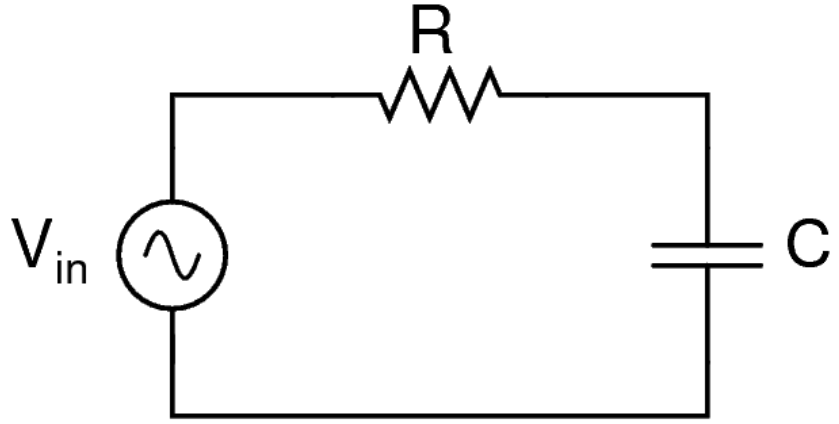
\includegraphics[scale = 0.3]{1.png}
\caption{RC Low Pass Filter}
\end{figure}


\subsection{Terminology}
\begin{enumerate}
\item \textbf{Time Constant (\(\tau)\):} The time taken by output voltage to rise by 63.2\% of the maximum output voltage
\item \textbf{Bandwidth (rad/s):} The
 reciprocal of the time constant i.e. \(\frac{1}{\tau}\)
 \item \textbf{Bandwidth (Hz):} The
 reciprocal of the time constant multiplied by 2\(\pi\) i.e. \(\frac{1}{2\pi\tau}\)
 \item \textbf{Rise Time (\(t_r\)):} Time taken for the signal to go from 10-90\% of its peak-to peak value
 \item \textbf{Fall Time (\(t_f\)):} Time taken for the signal to reach from 90-10\% of its peak-to peak value
\end{enumerate}

\subsection{Experimental results}
\begin{table}[!hbt]
		\begin{center}
		\begin{tabular}{|c|c|c|}
			\hline
			Sr. No. & Quantity & Value \\
			\hline
			1 & Time Constant (measured) & 66\(\mu\)s  \\
			\hline
			2 & Time Constant (calculated) & 100\(\mu\)s \\
			\hline
                3 & Bandwidth (measured) &  2.4 kHz \\
			\hline
                4 & Bandwidth (calculated) & 1.6 kHz  \\
			\hline
                5 & Rise Time (cursor) &  98.0\(\mu\)s \\
			\hline
                6 & Rise Time (measure) &  137.9\(\mu\)s \\
			\hline
                7 & Fall Time (cursor) &  170\(\mu\)s \\
			\hline
                8 & Fall Time (measure) &  146.6\(\mu\)s \\
			\hline
		\end{tabular}
        
		\end{center}
\end{table}

\begin{figure}[h!]
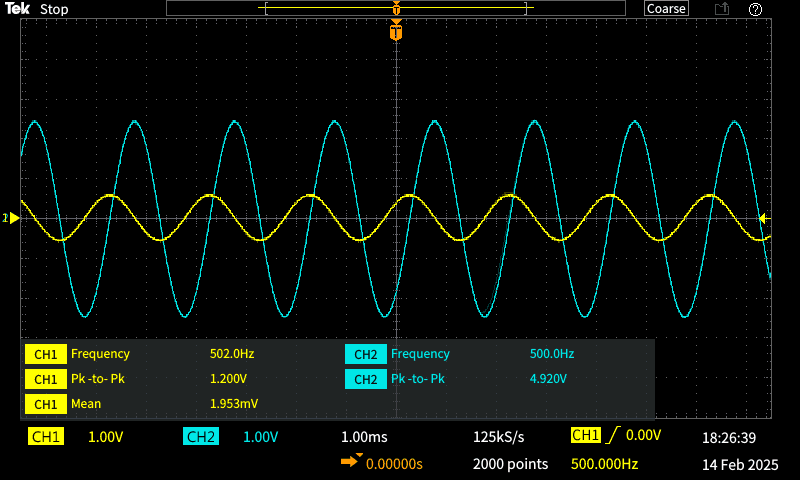
\includegraphics[scale = 0.7, center]{TEK00004.PNG}
\caption{\raggedright Output Waveform}
\end{figure}
\begin{figure}[h!]
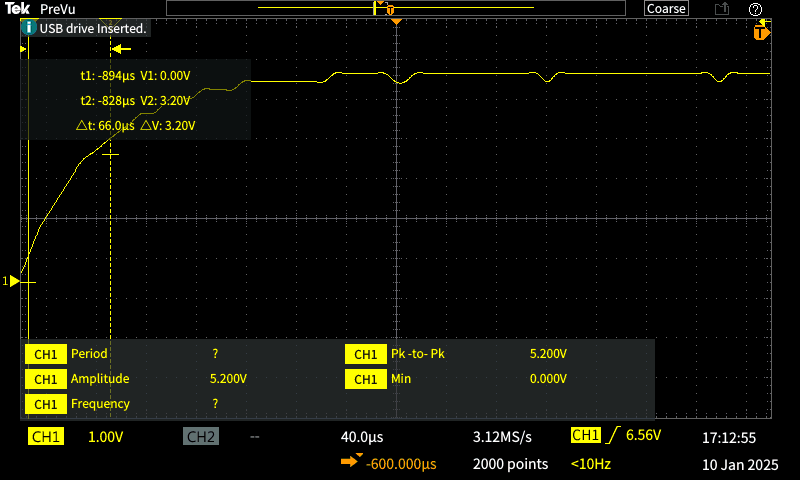
\includegraphics[scale = 0.5, center]{TEK00001.PNG}
\caption{\raggedright Calculation of the Time Constant}
\end{figure}
\newpage
\vspace*{1.5cm}
\begin{figure}[h!]
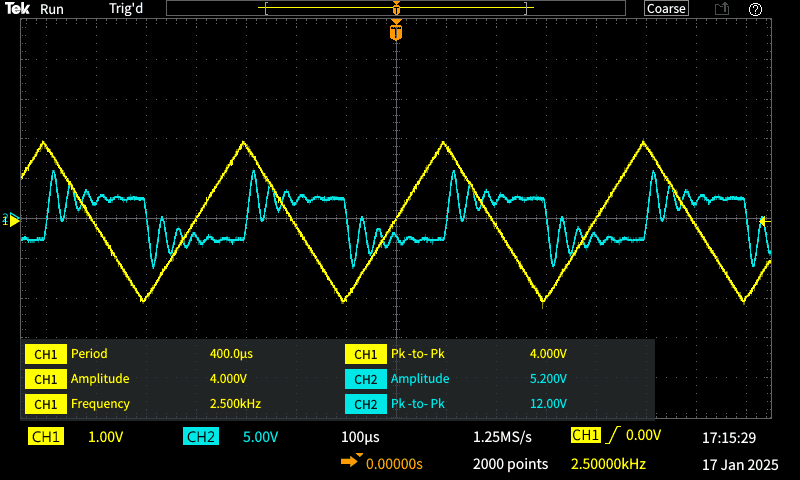
\includegraphics[scale = 0.5, center]{TEK00002.PNG}
\caption{\raggedright Calculation of the Rise Time (Cursor)}
\newpage
\end{figure}
\begin{figure}[h!]
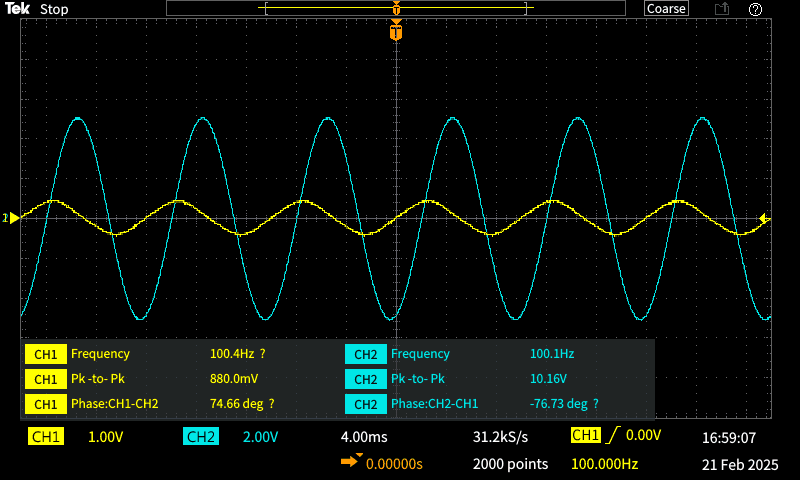
\includegraphics[scale = 0.5, center]{TEK00003.PNG}
\caption{\raggedright Calculation of the Fall Time (Cursor)}
\end{figure}
\newpage
\vspace*{1cm}
\begin{figure}[h!]
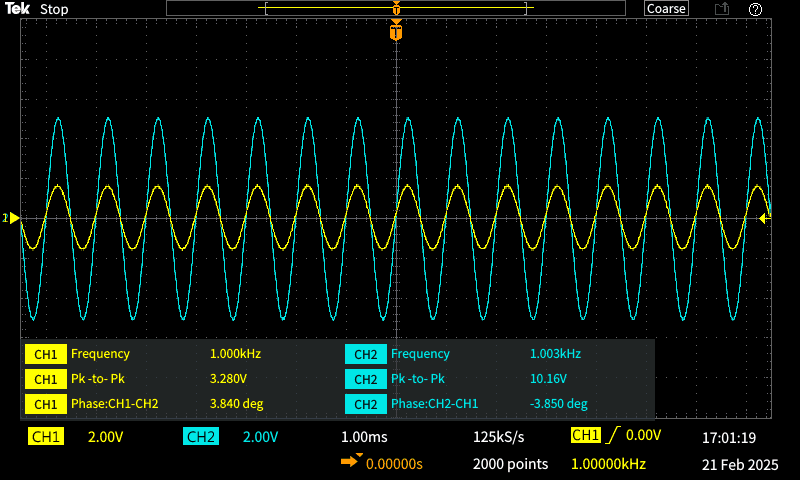
\includegraphics[scale = 0.5, center]{TEK00005.PNG}
\caption{\raggedright Calculation of the Rise and Fall Time (Measure)}
\end{figure}


\subsection{Conclusion and Inference}
\begin{enumerate}
\item The waveform corresponds to the charging and discharging of the capacitor across the resistor. During the charging phase, the slope of the graph is high and as the capacitor gets charged, the graph's slope becomes almost 0 and the same goes for discharging of the capacitor.
\item The huge difference between the measured and calculated values of bandwidth is because of the non-ideal nature of the capacitor in real life due to which its working capacitance varies significantly and causes such ginormous error in the bandwidth.
\item The results for Rise Time and Fall Time from Cursor and Measure are different but are also in each other's vicinity which is due to the fact that Cursor uses points in vicinity of the actual value points to get the values and at these small scales, even small perturbations lead to significant deviation from the actual value.
\item This experiment showcases the importance of accurate and precise measurements, errorless instruments and the use of ingenuity while experimenting to figure out where its going wrong. Other than that, it covered the part which was already taught in earlier courses with extra info about Rise Time and Fall Time. We also learnt how to use the DSO, the AFG and how to work around errors and difficulties which arise during experimentation. 
\end{enumerate}


\subsection{Experiment completion status}
The complete experiment was performed in front of the TA in the lab itself.
% ----------------------------------------------------------------------------------


\newpage
\section{Frequency response of RC circuit}
\subsection{Aim of the experiment}
To study the frequency response of an RC low-pass filter circuit and determine its amplitude-frequency characteristics. Specifically:

\begin{enumerate}
\item \textbf{Amplitude-Frequency Response:} Measure and analyze the output amplitude (\( V_{outpp} \)) at various input frequencies, starting from 5 Hz and increasing up to 1 MHz in decade steps, using a sinusoidal input signal of 1 \( V_{pp} \) and then record the results and plot the Bode plot.

\item \textbf{Bandwidth Determination:} Identify the bandwidth of the RC circuit by locating the frequency range where the output amplitude decreases to \( \frac{1}{\sqrt{2}} \) (approximately -3 dB) of the input amplitude.

\item \textbf{Comparison and Analysis:} Compare the experimentally measured bandwidth with the theoretical bandwidth calculated using the circuit's time-domain response and provide explanations for any discrepancies or observations.
\end{enumerate}

\subsection{Design}
The design of the circuit requires us to assemble all the required circuit elements on a breadboard and connect them to the Arbitrary Function Generator and probe the circuit using Digital Storage Oscilloscope.  \\
\hspace*{1cm}  After doing the mesh analysis of the given circuit, we get the following equation, with \textit{i} being the current in the circuit: 

\begin{equation}
     V_{in}
        \\
     = iR + \frac{1}{C}\int idt   
\end{equation}     

\begin{figure}[h!]
\centering
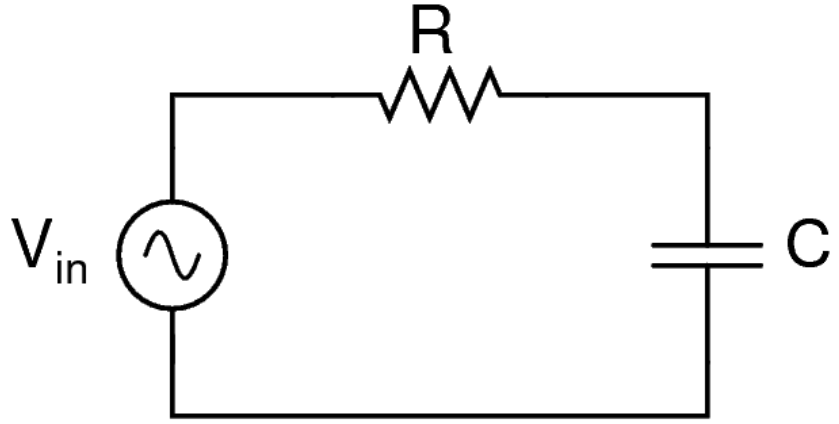
\includegraphics[scale = 0.3]{1.png}
\caption{RC Low Pass Filter}
\end{figure}

\subsection{Terminology}
\begin{enumerate}
\item \textbf{Amplitude-Frequency response (Bode Plot):} A graphical representation of the system's frequency response, showing how the magnitude (gain) and phase shift of the current change with respect to the voltage at different frequencies
\item \textbf{Bandwidth (Hz):} The frequency range in which the output of a circuit reaches \(\frac{1}{\sqrt{2}}\) times the amplitude of the input signal, often corresponding to a -3 dB reduction in output amplitude
\end{enumerate}

% \subsection{Simulation results}
\subsection{Experimental results}
\begin{table}[!hbt]
		\begin{center}
		\begin{tabular}{|c|c|c|}
			\hline
			Sr. No. & Frequency  & \(V_{PP}\) (mV) \\
			\hline
			1 & 5 Hz & 1000  \\
			\hline
                2 & 50 Hz & 1000  \\
			\hline
                3 & 200 Hz & 1000  \\
			\hline
                4 & 1 kHz & 900  \\
			\hline
                5 & 2 kHz & 652  \\
			\hline
                6 & 3 kHz &  500 \\
			\hline
                7 & 5 kHz &  364 \\
			\hline
                8 & 10 kHz &  208 \\
			\hline
                9 & 20 kHz &  108 \\
			\hline
                10 & 30 kHz &  76 \\
			\hline
                11 & 40 kHz &  58 \\
			\hline
                12 & 50 kHz &  45.6 \\
			\hline
                13 & 60 kHz & 36  \\
			\hline
                14 & 70 kHz &  33.6 \\
			\hline
                15 & 80 kHz & 28.8  \\
			\hline
                16 & 90 kHz &  21.6 \\
			\hline
                17 & 100 kHz & 18.4  \\
			\hline
                18 & 200 kHz & 12  \\
			\hline
                19 & 300 kHz & 8.8  \\
			\hline
                20 & 400 kHz &  7.8 \\
			\hline
                21 & 500 kHz & 5  \\
			\hline
                22 & 600 kHz & 4  \\
			\hline
                23 & 700 kHz & 3.2  \\
			\hline
                24 & 800 kHz &  2.4 \\
			\hline
                25 & 900 kHz &  2 \\
			\hline
                26 & 1 Mhz &  1.4 \\
			\hline
		\end{tabular}
		\end{center}
\end{table}
\begin{table}[!hbt]
		\begin{center}
		\begin{tabular}{|c|c|c|}
			\hline
			Sr. No. & Quantity & Value \\
			\hline
			1 & Bandwidth (measured) & 1.8 kHz  \\
			\hline
			2 & Bandwidth (calculated) & 1.6 kHz \\
			\hline
		\end{tabular}
        
		\end{center}
\end{table}
\newpage
\begin{figure}[h!]
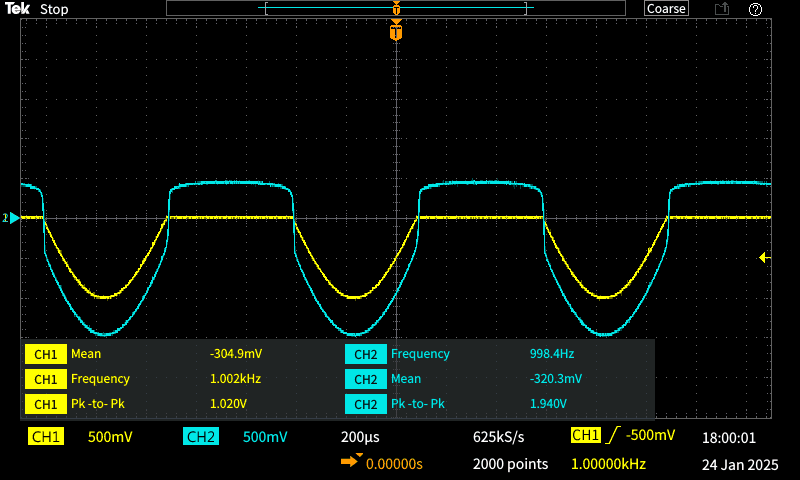
\includegraphics[scale = 0.5, center]{TEK00006.PNG}
\caption{\raggedright Output Waveform at 5 Hz }
\end{figure}
\vspace*{1.5cm}
\begin{figure}[h!]
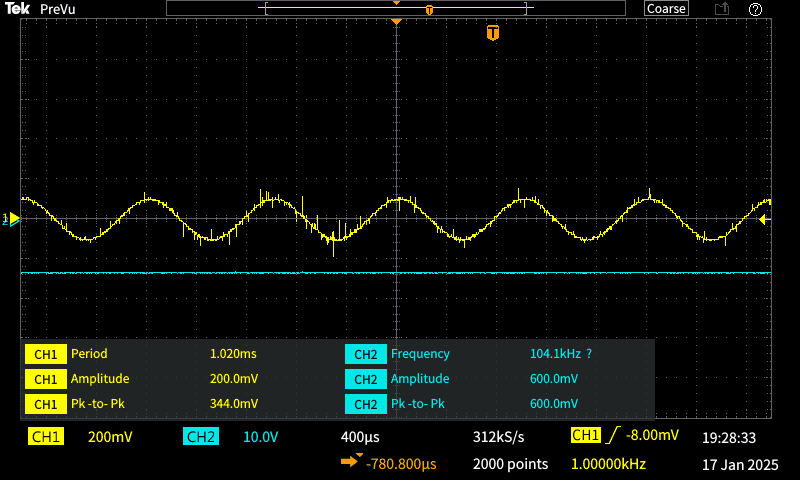
\includegraphics[scale = 0.5, center]{TEK00018.PNG}
\caption{\raggedright Output Waveform at 100 kHz}
\end{figure}
\newpage
\begin{figure}[h!]
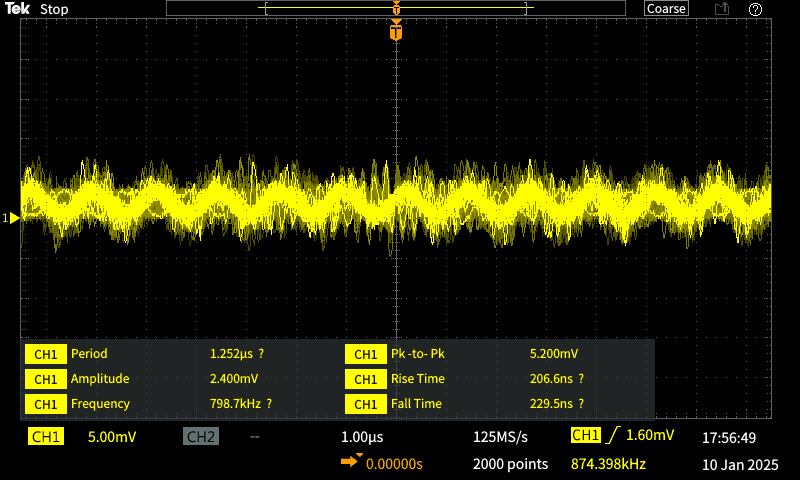
\includegraphics[scale = 0.5, center]{TEK00026.PNG}
\caption{\raggedright Output Waveform at 800 kHz}
\end{figure}
\subsection{Conclusion and Inference}
\begin{enumerate}
\item The deviation of the measured Bandwidth from the calculated Bandwidth is because of the non-ideal behavior of the various components of the circuit especially the capacitor which just disturbs the mean Bandwidth of the circuit. 
\item The experiment also shows how small errors add up over time to change the output so much that it becomes irrecognizable like in the case of measured and calculated Bandwidths. It also gives insights into the Bode plot method of the evaluation of various parameters of a system. 
\end{enumerate}
\subsection{Experiment completion status}
All the activities of the experiment were completed in the lab itself with utmost care and diligence. 
% ----------------------------------------------------------------------------------


\newpage
\section{Basics of probing the circuit}
\subsection{Aim of the experiment}
To understand the basics of circuit probing using a potential divider circuit and demonstrate correct methods of measuring electrical signals. Specifically:

\begin{enumerate} 
\item Measure the voltage across \( R_{3}\) and compare it with the expected value.
\item Measure the voltage across \( R_{2}\) without removing the connection across \( R_{3}\), compare results, and explain the cause of error.
\item Identify the appropriate instrument to avoid this error.
\item Apply a sinusoidal input across the potential divider, measure the voltage waveform across \( R_{2}\), and compare it with the expected waveform.
\end{enumerate}

\subsection{Design}
The experiment requires us to arrange the resistors in the given manner on the breadboard and then applying voltages of \( V_{DD} = + 15 V \) and \( V_{SS} = - 15 V \) in the first part followed by a sinusoidal input of \( 5\;V_{PP} \) at \( 4.7\;KHz \) from the AFG. The equations describing the workings of the circuit is:  
\begin{equation}
     V_{DD} - V_{SS}
        \\
     = i(R_{1} + R_{2} + R_{3}) 
\end{equation} 

\begin{figure}[h!]
\centering
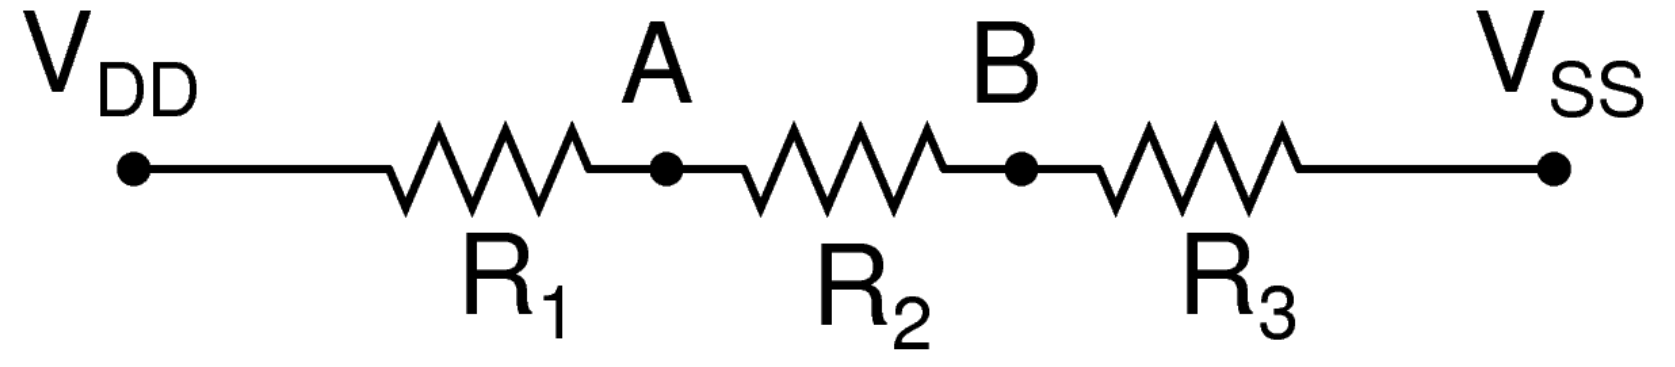
\includegraphics[scale = 0.2]{3.png}
\caption{Potential Divider Circuit}
\end{figure}

% \subsection{Simulation results}
\subsection{Experimental results}
\begin{table}[!hbt]
		\begin{center}
		\begin{tabular}{|c|c|c|}
			\hline
			Sr. No. & Quantity  &  Value\\
			\hline
                 1 & \(V_{R_3}\) (measured) & 10.11 V (DC) \\
			\hline
                 2 & \(V_{R_3}\) (calculated) & 10 V (DC) \\
			\hline
                 3 & \(V_{R_2}\) (measured) & 19.77 V (DC)\\
			\hline
                 4 & \(V_{R_2}\) (calculated) & 10 V (DC)\\
			\hline
                 5 & \(V_{R_2}\) (measured)  & 2.8 V (AC) \\
			\hline
                 6 & \(V_{R_2}\) (calculated) & 1.66 V (AC) \\
			\hline
		\end{tabular}
        
		\end{center}
\end{table}
\newpage
\begin{figure}[h!]
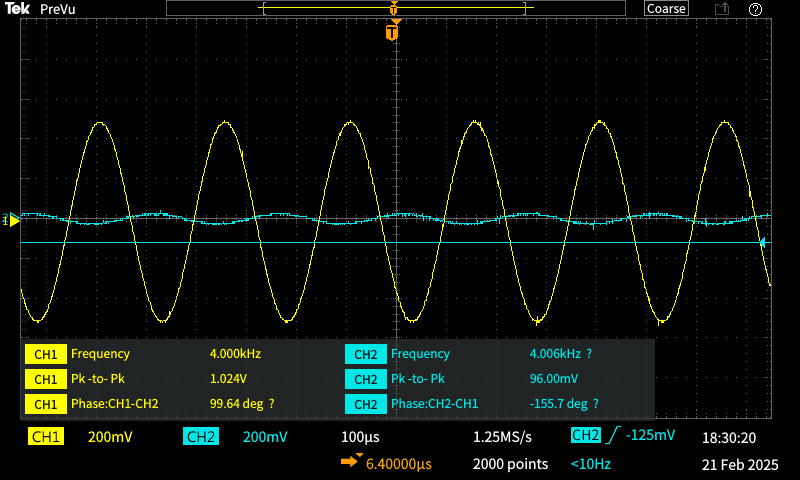
\includegraphics[scale = 0.5, center]{TEK00028.PNG}
\caption{\raggedright DC Voltage across \(R_3\) at CH1}
\end{figure}
\vspace*{1.5cm}
\begin{figure}[h!]
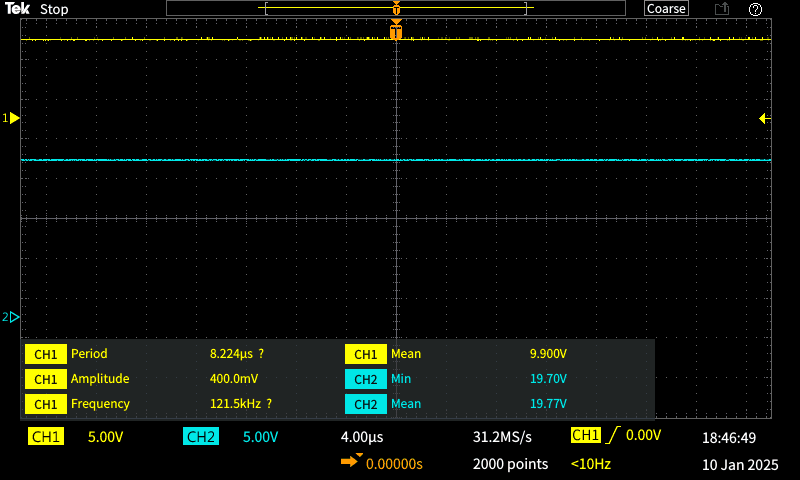
\includegraphics[scale = 0.5, center]{TEK00030.PNG}
\caption{\raggedright DC Voltage across \(R_2\) at CH2}
\end{figure}
\newpage
\begin{figure}[h!]
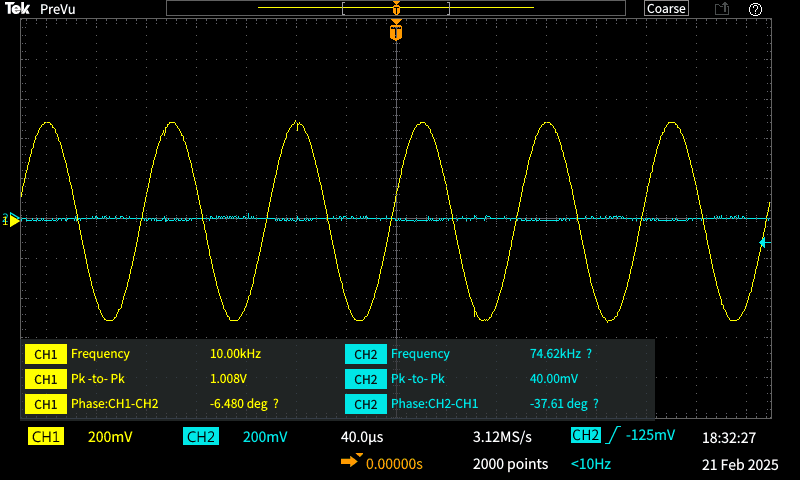
\includegraphics[scale = 0.5, center]{TEK00031.PNG}
\caption{\raggedright AC Voltage across \(R_2\) at CH1  }
\end{figure}

\subsection{Conclusion and Inference}
\begin{enumerate}
\item The expected value and calculated values of voltage across \(R_3\) are similar with a small discrepancy arising due to inaccurate instruments, the resistance of wires and the voltage fluctuation by the source. The non-ideal behavior of resistors also contributes to the above cause.
\item The voltage gap between the measured value and the calculated value of \(R_2\) arises due to the internal connections of the DSO. To measure the voltage across the second resistor, we end up shorting the third one and thus the effective resistance of the circuit becomes 20 \(\Omega\), leading to the significant rise in the voltage at \(R_2\).
\item We can avoid the above error by using a high-impedance probe such as 10x or 100x attenuation probe with DSO which reduces the loading effect and thereby reduces the error.
\item Again the measured and calculated values differ because of the loading effect and internal flaws of the circuit.

\end{enumerate}
\subsection{Experiment completion status}
All the parts of the experiment were done in the lab itself and nothing was left for later.
% ----------------------------------------------------------------------------------


\newpage
\section{Half wave Rectifier}
\subsection{Aim of the experiment}
To analyze the operation of a half-wave rectifier circuit using a sinusoidal input signal. \\Specifically:
\begin{enumerate}
\item Observe and plot the input and output waveforms using a DSO.
\item Explain the reduction in peak amplitude between the input and output voltages.
\item Reverse the diode polarity, observe the changes, and explain the resulting waveforms.
\end{enumerate}

\subsection{Design}
The experiment uses key components including a 1N4007 diode, a 22 kΩ resistor, a signal generator to apply a sinusoidal input of 4 \(V_{PP}\) at 1 kHz, and a digital storage oscilloscope (DSO) to observe and plot the input (\(V_{i} \)) and output (\(V_{o} \)) waveforms. The circuit is arranged with the diode in series with the resistor, forming a simple half-wave rectifier. The anode of the diode is connected to the input source, while the cathode is connected to one end of the resistor. The output is measured across the resistor using the DSO.\\
\hspace*{2cm} The following equations describe the circuit:
\begin{equation}
     V_{out} = V_{in}  \hspace{2cm} \text{(Diode On)}   
\end{equation} 

\begin{equation}
     V_{out} = 0   \hspace{2.5cm} \text{(Diode Off)}   
\end{equation} 

\begin{figure}[h!]
\centering
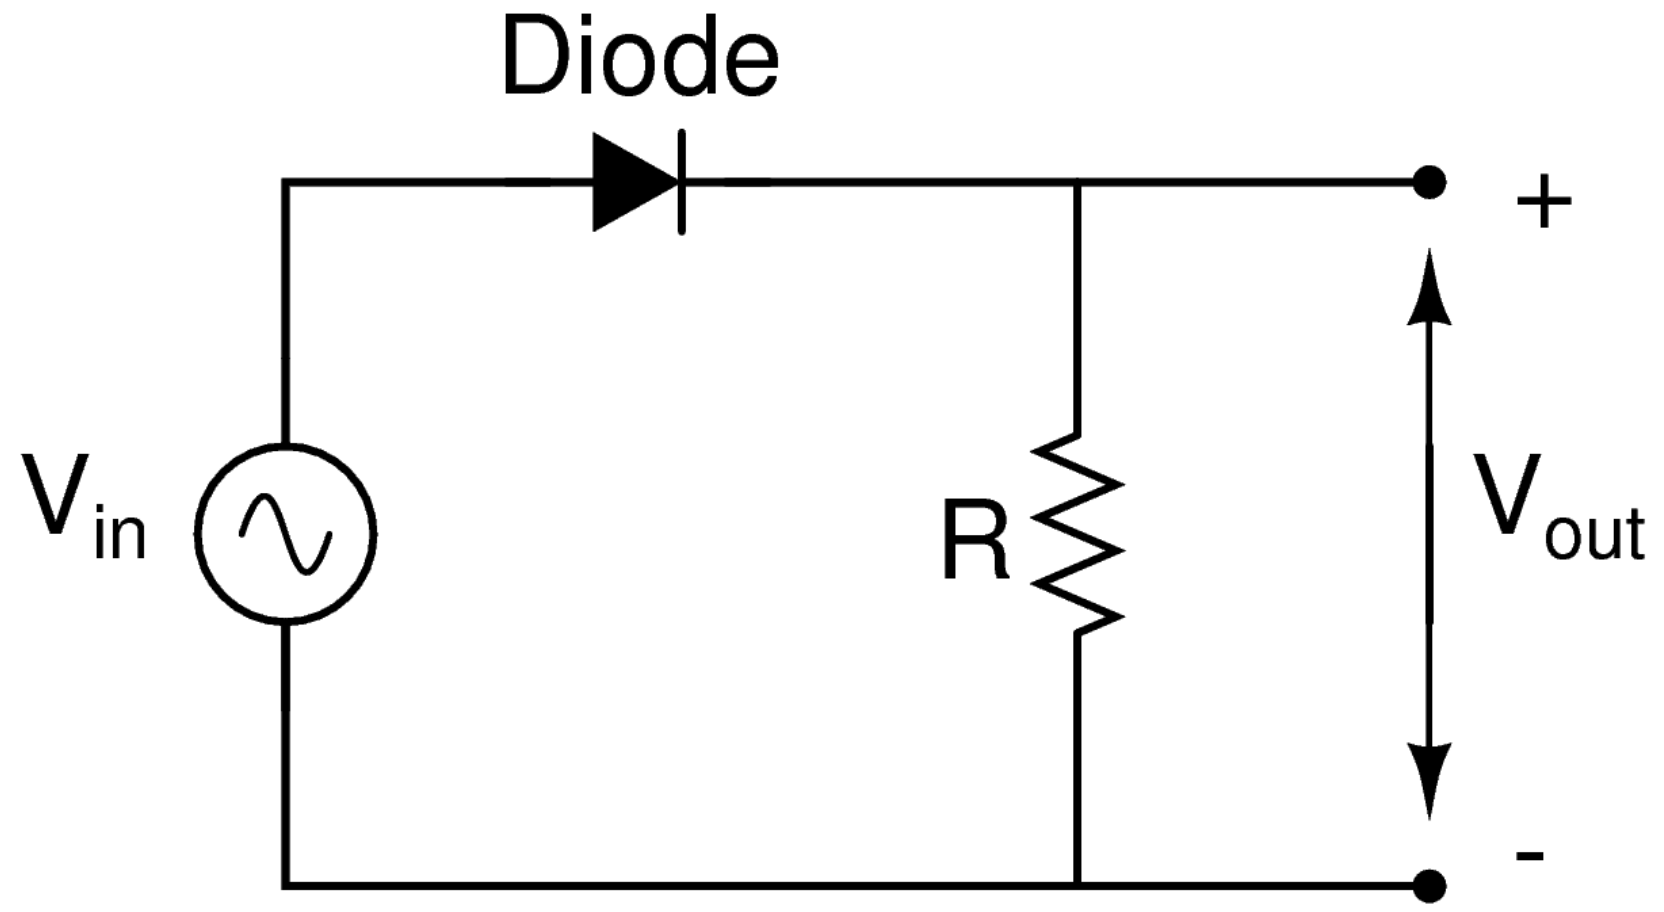
\includegraphics[scale = 0.2]{4.png}
\caption{Half Wave Rectifier}
\end{figure}
\newpage
% \subsection{Simulation results}
\subsection{Experimental results}
\begin{figure}[h!]
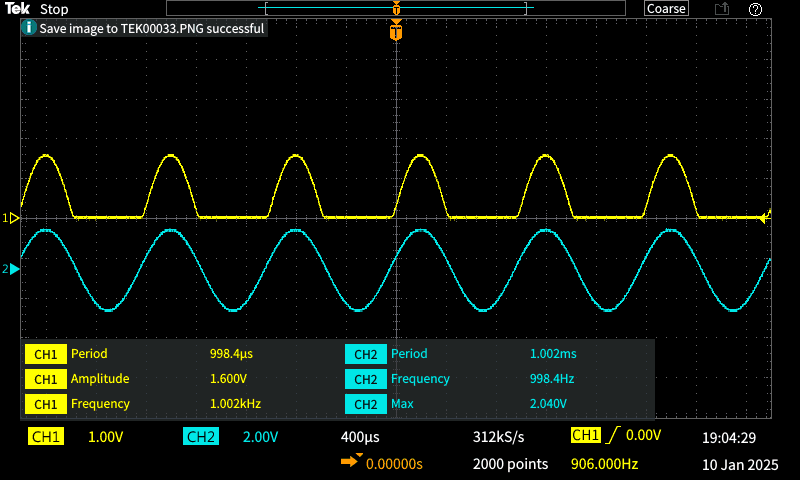
\includegraphics[scale = 0.5, center]{TEK00034.PNG}
\caption{\raggedright \(V_o\) and \(V_i\) against \textit{t}}
\end{figure}
\vspace*{1.5cm}
\begin{figure}[h!]
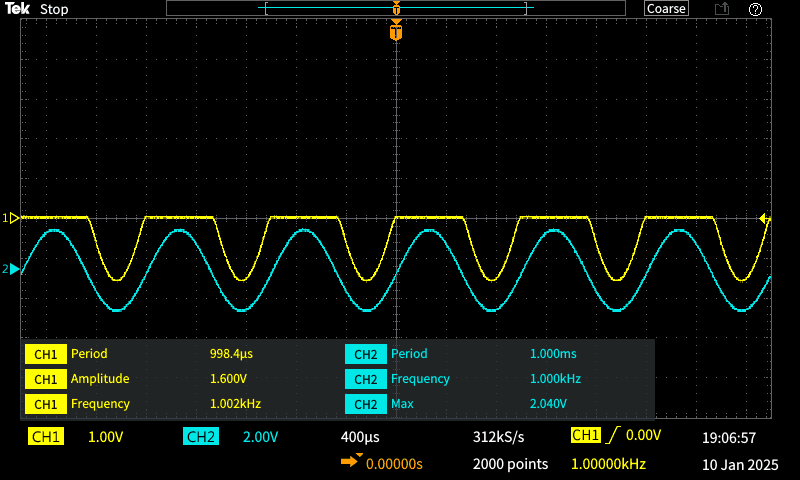
\includegraphics[scale = 0.5, center]{TEK00035.PNG}
\caption{\raggedright \(V_o\) and \(V_i\) against \textit{t} after  change of polarity of diode}
\end{figure}

\subsection{Conclusion and Inference}
\begin{enumerate}
\item The reduction in the peak amplitude between the input and the output voltage is attributed to the diode drop which is the voltage required to overcome the internal voltage barrier of the diode. 
\item Now, by changing the polarity of the diode, the direction in which the current flows gets reversed and the graph of \(V_{out}\) gets flipped across the x-axis leading to only negative voltages at the output terminal.
\end{enumerate}
\subsection{Experiment completion status}
The experiment, in its entirety was completed in the lab itself with some help from the intelligent and very kind TA.
% ----------------------------------------------------------------------------------


\newpage
\section{OpAmp based negative feedback circuits - Non Inverting Amplifier}
\subsection{Aim of the experiment}
To study the operation of an inverting amplifier circuit by analyzing its input and output waveforms. Specifically:

\begin{enumerate}
\item Plot the input and output waveforms for a sinusoidal input of 0.1 V peak at 1 kHz and observe the circuit's behavior.
\item Vary the input amplitude from 0.1 V to 2 V, observe changes in the output waveform, and explain the behavior of the output voltage beyond a certain input threshold.
\end{enumerate}

\subsection{Design}
The experiment involves an inverting amplifier circuit using an operational amplifier (OpAmp) powered by a ±15 V dual supply. Key components include resistors \(R_{1} \)=1 kΩ and \(R_{2} \)=10 kΩ, a signal generator to provide a sinusoidal input with an initial peak amplitude of 0.1 V at 1 kHz, and a digital storage oscilloscope (DSO) for plotting input (\(V_{i} \)) and output (\(R_{o} \)) waveforms. The circuit is arranged with \(R_{1} \) connected between the input signal and the inverting terminal of the op-amp, and \(R_{2} \) providing feedback between the output and the inverting terminal. The non-inverting terminal is grounded. The output is measured directly on the DSO, which serves as the load. Changes in input amplitude from 0.1 V to 2 V are applied, and the corresponding output waveforms are observed and analyzed.
\begin{equation}
     V_{o} = V_{i}(1 + \frac{R_{2}}{R_{1}})   \hspace{2cm} \text{(Operating Mode)}
\end{equation}     
\begin{equation}
     V_{o} = ± 15V   \hspace{3.2cm} \text{(Saturation Mode)}
\end{equation}     

\begin{figure}[h!]
\centering
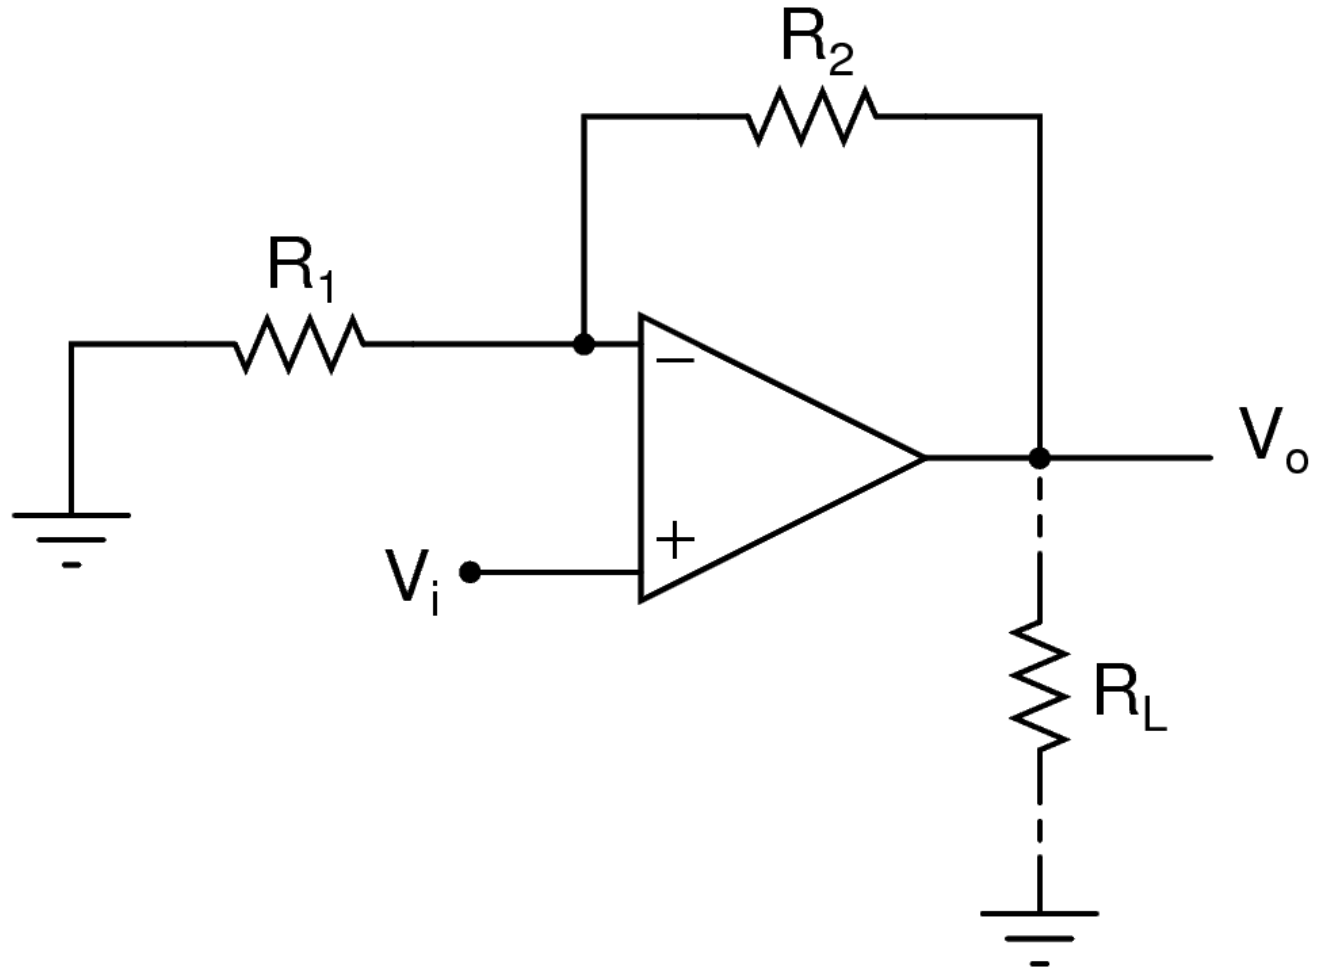
\includegraphics[scale = 0.25]{5.png}
\caption{Non-Inverting Amplifier}
\end{figure}

% \subsection{Simulation results}
\subsection{Experimental results}
\begin{figure}[h!]
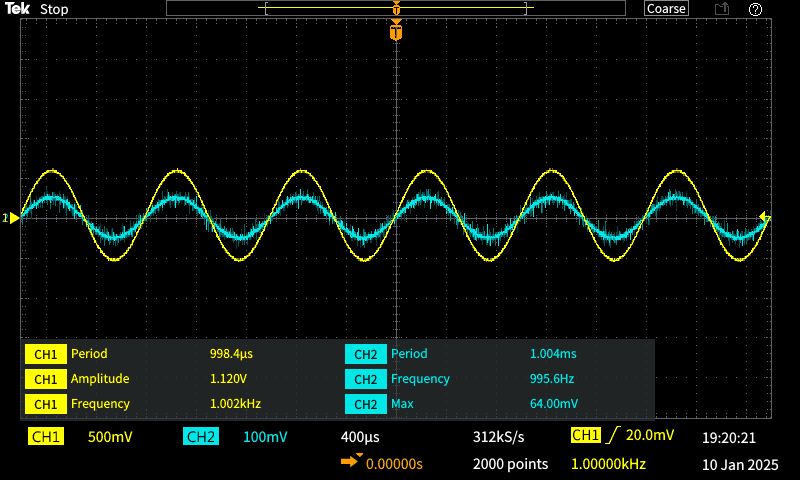
\includegraphics[scale = 0.5, center]{TEK00036.PNG}
\caption{\raggedright \(V_o\) and \(V_i\) against \textit{t}}
\end{figure}
\vspace*{1.5cm}
\begin{figure}[h!]
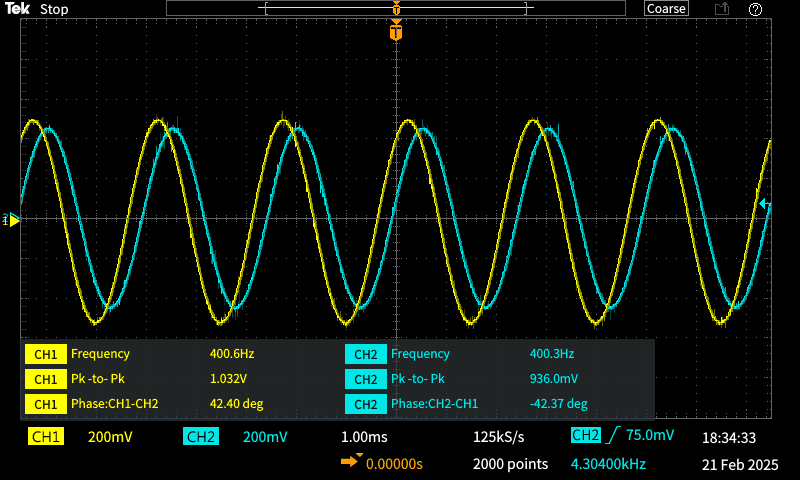
\includegraphics[scale = 0.5, center]{TEK00037.PNG}
\caption{\raggedright \(V_o\) and \(V_i\) against \textit{t} at $|$\(V_i\)$|$ = 2 V}
\end{figure}

\subsection{Conclusion and Inference}
\begin{enumerate}
\item By changing the input amplitude from 0.1 V to 2 V, we exceed the voltage threshold for the amplifier and it goes into the saturation mode, outputting a voltage of 15 V regardless of the input voltage. 
\end{enumerate}
\subsection{Experiment completion status}
Each and every part of this very long experiment was performed by me at the lab and nothing was left for later. 

\end{document}

\begin{table}[!hbt]
		\begin{center}
		\begin{tabular}{|c|c|c|}
			\hline
			     &  &  \\
			\hline
                  &  &  \\
			\hline
                  &  &  \\
			\hline
                  &  &  \\
			\hline
                  &  &  \\
			\hline
                  &  &  \\
			\hline
		\end{tabular}
        
		\end{center}
\end{table}
